\documentclass[article,shortnames]{jss}
\usepackage[utf8]{inputenc}
\usepackage{natbib}
\usepackage{pdfpages}
\usepackage{xspace}
\usepackage{array}
\usepackage{tikz}
\usetikzlibrary{shapes.geometric, arrows}

\tikzstyle{io} = [trapezium, trapezium left angle=70, trapezium right angle=110, minimum width=3cm, minimum height=1cm, text centered, draw=black, fill=blue!30]
\tikzstyle{process} = [rectangle, minimum width=3cm, minimum height=1cm, text centered, draw=black, fill=orange!30]
\tikzstyle{decision} = [diamond, minimum width=3cm, minimum height=1cm, text centered, draw=black, fill=green!30]
\tikzstyle{arrow} = [thick,->,>=stealth]

\newcommand{\hl}[1]{\textcolor{magenta}{#1}}

\renewcommand\topfraction{.9}
\renewcommand\textfraction{.1}
\renewcommand{\floatpagefraction}{.6}
\renewcommand{\topfraction}{0.85}
\renewcommand{\bottomfraction}{0.85}
\renewcommand{\textfraction}{0.15}
\renewcommand{\floatpagefraction}{0.7}

%Virker ikke:
%\newcommand{\R}{\proglang{R}\xspace}

\newcommand{\R}[1]{\code{#1}}

\newcolumntype{L}[1]{>{\raggedright\let\newline\\\arraybackslash\hspace{0pt}}p{#1}}
\newcolumntype{C}[1]{>{\centering\let\newline\\\arraybackslash\hspace{0pt}}p{#1}}
\newcolumntype{R}[1]{>{\raggedleft\let\newline\\\arraybackslash\hspace{0pt}}p{#1}}


%%%%%%%%%%%%%%%%%%%%%%%%%%%%%%
%% declarations for jss.cls %%%%%%%%%%%%%%%%%%%%%%%%%%%%%%%%%%%%%%%%%%
%%%%%%%%%%%%%%%%%%%%%%%%%%%%%%

%% almost as usual
\author{Anne H. Petersen\\Biostatistics\\Department of Public
  Health\\University of Copenhagen \And Claus Thorn Ekstr\o m\\Biostatistics\\Department of Public
  Health\\University of Copenhagen}
\title{\pkg{dataMaid}: your assistant for data cleaning in \proglang{R}}

%% for pretty printing and a nice hypersummary also set:
\Plainauthor{Anne H. Petersen, Claus Thorn Ekstr\o m} %% comma-separated
\Plaintitle{{dataMaid}: your assistant for data cleaning in R} %% without formatting
\Shorttitle{\pkg{dataMaid}: your data cleaning personal assistant in R} %% a short title (if necessary)

%% an abstract and keywords
\Abstract{Data cleaning and -validation are the first steps in any
  data analysis, as the validity of the conclusions from the analysis
  hinges on the quality of the input data. Mistakes in the data can
  arise for any number of reasons, including erroneous codings,
  malfunctioning measurement equipment, and inconsistent data generation
  manuals.  Ideally, a human investigator should go
  through each variable in the dataset and look for potential errors
  --- both in input values and codings --- but that process can be very
  time-consuming, expensive and error-prone in itself.

  We describe an \proglang{R} package, \pkg{dataMaid}, which
  implements an extensive and customizeable suite of quality
  assessment tools that can be applied to a dataset in order to
  identify potential problems in its variables. The results can be
  presented in an auto-generated, non-technical, stand-alone overview
  document intended to be perused by an investigator with an
  understanding of the variables in the data, but not necessarily
  knowledge of \proglang{R}. Thereby, \pkg{dataMaid} aids the dialogue
  between data analysts and field experts, while also providing easy
  documentation of reproducible data cleaning steps and data quality
  control. Moreover, the \pkg{dataMaid} solution changes the data
  cleaning process from the usual ad hoc approach to a systematic,
  well-documented endeavor.  \pkg{dataMaid} also provides a suite of
  more typical \proglang{R} tools for interactive data quality
  assessment and -cleaning, where the data inspections all live and
  die within the \proglang{R} console.

  % The \pkg{dataMaid} package is designed to be easily extended with
  % custom user-created checks that are relevant in particular
  % situations. \hl{Already said that above. Either expand on it or
  % delete this.}
}
\Keywords{data cleaning, quality control, \proglang{R}}
\Plainkeywords{data cleaning, quality control, R} %% without formatting
%% at least one keyword must be supplied

%% publication information
%% NOTE: Typically, this can be left commented and will be filled out by the technical editor
%% \Volume{50}
%% \Issue{9}
%% \Month{June}
%% \Year{2012}
%% \Submitdate{2012-06-04}
%% \Acceptdate{2012-06-04}

%% The address of (at least) one author should be given
%% in the following format:
\Address{
  Claus Thorn Ekstr\o m\\
  Biostatistics, Department of Public Health\\
  University of Copenhagen\\
  Denmark\\
  E-mail: \email{ekstrom@sund.ku.dk}\\
  URL: \url{http://staff.pubhealth.ku.dk/~ekstrom/}
}
%% It is also possible to add a telephone and fax number
%% before the e-mail in the following format:
%% Telephone: +43/512/507-7103
%% Fax: +43/512/507-2851

%% for those who use Sweave please include the following line (with % symbols):
%% need no \usepackage{Sweave.sty}

%% end of declarations %%%%%%%%%%%%%%%%%%%%%%%%%%%%%%%%%%%%%%%%%%%%%%%


\begin{document}


\section{Introduction}
Though data cleaning might be regarded as a somewhat tedious activity,
adequate data cleaning is crucial in any data analysis. With
ever-growing dataset sizes and complexities, statisticians and data
analysts find themselves spending a large portion of their time on
data cleaning and data wrangling. While a computer should never
make unsupervised decisions on what should be done to potential
errors in a dataset, it can still be an extremely useful tool in the
data cleaning process. Some errors can be tracked down and flagged by a
computer without further ado, while other types of errors need an analytic
context in order to be identified. Even in this latter case, well-designed
software can aid the process tremendously by providing the human
investigator with the
information needed for identifying issues.


A number of \proglang{R} packages made for such pre-analysis tools are
already available, including \pkg{janitor} \citep{janitor}, \pkg{plyr}
\citep{plyr}, \pkg{data.table} \citep{data.table}, \pkg{DataCombine}
\citep{DataCombine} , \pkg{validate} \citep{validate}, and
\pkg{DataExplorer} \citep{DataExplorer}. These packages focus on
different stages of the pre-analysis work, most of which are not
really data cleaning.  \pkg{janitor} provides tools for data import
with a particular emphasis on the challenges of getting neat data
frames from Microsoft Excel data files. \pkg{plyr}, \pkg{data.table}
and \pkg{DataCombine} go a few steps further by providing a wide array
of extremely powerful tools for data wrangling, including a number of
particularly useful functions for merging and working with very large
datasets. When it comes to actual data cleaning, however, the options
are fewer.  \pkg{validate} (and the similar packages \pkg{editrules}
\citep{editrules} and \pkg{deducorrect} \citep{deducorrect} from the
same authors) does offer a few tools for identifying and
auto-correcting errors in a dataset, but, as the name suggests, the
focus is on internal validity rather than general data cleaning. In
practice, this means that quite elegant tools for, e.g., linear
restraints among the variables in a dataset can be applied, but
looking for potentially miscoded missing values is not really
feasible. The main difference between these two challenges is the
direction in which the data is inspected: While linear constraints
work row-wise with no ambiguity, determining whether or not something
is a miscoded missing value often requires knowledge about the full
variable (e.g. range or data type), and thus it should be performed
column-wise. \pkg{validate} does not allow for user-defined extensions
of the latter type, thereby limiting its data cleaning potential.
Automatic data correction functions are also provided by
\pkg{validate} which we consider to be quite a dangerous cocktail: all
power is given to the the computer with no human supervision, and
investigators are less likely to make an active, case-specific choice
regarding the handling of the potential errors.  Finally, no tools
have been made to easily document exactly which checks and preliminary
results were used in the data cleaning process.

All in all, the large role of data cleaning in any data analysts
everyday endeavors is hardly matched in the amount of available
\proglang{R} software solutions. In particular, few packages attempt
to implement systematic, reproducible data cleaning. And while the
available tools attempt to alleviate the ubiquitous ad hoc approach to
data cleaning, they are primarily intended for the data savvy users
and less so for the general researcher with a knowledge about a
specific field and the context of the available data. The
\pkg{dataMaid} package \citep{dataMaid} presented here tries to address this by
providing a framework that both allows for extendable, systematic,
reproducible data cleaning, and summarizing findings for researchers
from other fields such that they can act as human experts when
tracking down potential errors.


One last package that should be mentioned in this context is
\pkg{DataExplorer} \citep{DataExplorer}. While this package does not
address data cleaning issues \emph{per se}, its general strategy is
quite similar to that of \pkg{dataMaid} and to the paradigms presented
below. This package provides a few simple, but practical, tools for
exploratory data analysis, including automated
documentation. Therefore, we find \pkg{DataExplorer} to be a good
candidate for a next-step package after data cleaning is finished.

But no matter how clever software tools we make, data cleaning remains
to be a time consuming endeavor, as it inherently requires human
interaction since every dataset is different and the variables in the
dataset can only be understood in the proper context of their
origin. This often requires a collaborative effort between an expert
in the field and a statistician or data scientist, which may be why
the process of proper data cleaning is not always undertaken. In many
situations, these errors are discovered in the process of the data
analysis (e.g., a categorical variable with numeric labels for each
category may be wrongly classified as a quantitative variable or a
variable where all values have erroneously been coded to the same
value), but in other cases a human with knowledge about the data
context area is needed to identify possible mistakes in the data
(e.g., if there are 4 categories for a variable that should only have
3).

The \pkg{dataMaid} approach to data cleaning and -quality assessment is
governed by two fundamental paradigms. First of all, there is no need
for data cleaning to be an ad hoc procedure. Often, we have a very
clear idea of what flags are raisable in a given dataset before we
look at it, as we were the ones to produce it in the first place. This
means that data cleaning can easily be a well-documented,
well-specified procedure. In order to aid this paradigm, \pkg{dataMaid}
provides easy-to-use, automated tools for data quality assessment in
\proglang{R} \citep{R} on which data cleaning decisions can be made. This quality
assessment is presented in an auto-generated overview document,
readable by data analysts and field experts alike, thereby also
contributing to an inter-field dialogue about the data at
hand. Oftentimes, e.g., distinguishing between faulty codings of a
numeric value and unusual, but correct, values requires
problem-specific expertise that might not be held by the data
analyst. Hopefully, having easy access to data descriptions through
\pkg{dataMaid} will help this necessary knowledge sharing.

While \pkg{dataMaid}s primary raison d'être is auto-generating data
quality assessment overview documents, we still wish to emphasize that
it is \emph{not} a tool for unsupervised data cleaning. This qualifies
as the second paradigm of \pkg{dataMaid}: Data cleaning decisions
should always be made by humans. Therefore, \pkg{dataMaid} does not
supply any tools for ``fixing'' errors in the data. However, we do
provide interactive functions that can be used to identify potentially
erroneous entries in a dataset and that can make it easier to solve
data issues, one variable at a time.


This manuscript is structured as follows: First, in Section
\ref{sec:usingdataMaid}, we introduce the main representative of the first
paradigm, namely the \code{clean()} function, which generates data
cleaning overview documents. In the \pkg{dataMaid} package, we have
provided a number of default cleaning steps that cover the data
cleaning challenges, we find to be most common. Next, in Section
\ref{sec:interactiveCleanR}, we present the interactive mode of \pkg{dataMaid}, as motivated
by the second paradigm above. But, as any data analyst knows,
every dataset is different, and some datasets might include problems
that cannot be detected by our data checking functions. In Section
\ref{sec:extending}, we turn to the question of how \pkg{dataMaid} extensions
can be made, such that they are integrable with the \code{clean()}
function and with the other tools available in \pkg{dataMaid}.  At last,
in Section \ref{sec:specificExamples}, we discuss a number of examples of
specific data cleaning challenges and how \pkg{dataMaid} can be used to
solve them.

% \hl{Is there a Section 6?}

%\hl{Do they typically discuss notation in articles like this? I try (somewhat inconsistently) to refer to functions as \R{function()} while other \R{R} objects are referred to merely as \R{object}. This is also the style adopted by Wickham in his books.}


%% include your article here, just as usual
%% Note that you should use the \pkg{}, \proglang{} and \code{}
%% commands.


\section{Creating a data cleaning overview}
\label{sec:usingdataMaid}

The \code{clean()} function is the primary workhorse of \pkg{dataMaid} and
this is the only function needed if a standard battery
of tests are used to generate data cleaning summaries. The data
cleaning summary itself is an overview document, intended for reading
by humans, in either pdf or html format. Appendix \ref{sec:appendix1}
provides an example of a data cleaning output document, produced by
calling \code{clean()} on the dataset \code{toyData} available in
\pkg{dataMaid}. The first two pages of this data cleaning output are
shown in Figure~\ref{fig:example1}. \code{toyData} is a very
small ($15$ rows of $6$ variables), artificial dataset which was created to
illustrate the main capabilities of \pkg{dataMaid}. The following
commands load the dataset and produce the cleaning output:

\begin{figure}[tb]
\begin{center}
\frame{\includegraphics[width=7.5cm,page=2]{dataMaid_toyData.pdf}}
\frame{\includegraphics[width=7.5cm,page=3]{dataMaid_toyData.pdf}}
%\includepdf[pages={2}, pagecommand={}]{dataMaid_testData.pdf}
\end{center}
\caption{Example output from running \code{clean()} on the \code{toyData}
  dataset. First a summary of the full dataset is given and then
  type-dependent information on each variable is given in a table and
  a graph. Larger versions of the pages can be seen in
  Appendix~\ref{sec:appendix1}.}
\label{fig:example1}
\end{figure}

\begin{Schunk}
\begin{Sinput}
R> library("dataMaid")
R> data("toyData")
R> toyData
\end{Sinput}
\begin{Soutput}
   var1 var2  var3       var4 var5       var6
1   red    1     a -0.6264538    1 Irrelevant
2   red    1     a  0.1836433    2 Irrelevant
3   red    1     a -0.8356286    3 Irrelevant
4   red    2     a  1.5952808    4 Irrelevant
5   red    2     a  0.3295078    5 Irrelevant
6   red    6     b -0.8204684    6 Irrelevant
7   red    6     b  0.4874291    7 Irrelevant
8   red    6     b  0.7383247    8 Irrelevant
9   red  999     c  0.5757814    9 Irrelevant
10  red   NA     c -0.3053884   10 Irrelevant
11 blue    4     c  1.5117812   11 Irrelevant
12 blue   82     .  0.3898432   12 Irrelevant
13 blue   NA       -0.6212406   13 Irrelevant
14 <NA>  NaN other -2.2146999   14 Irrelevant
15 <NA>    5 OTHER  1.1249309   15 Irrelevant
\end{Soutput}
\end{Schunk}
\begin{Schunk}
\begin{Sinput}
R> clean(toyData)
\end{Sinput}
\end{Schunk}

By default, an \proglang{R} markdown file and a rendered pdf overview
document is produced, saved to the working directory and
opened for immediate inspection. Turning to Figure~\ref{fig:example1},
we see that such a data cleaning output document consists of two
parts. First, an overview of what was done is presented under the
title \textit{Data cleaning summary}. Secondly, each variable in the
dataset is presented in turn using (up to) three tools in the
\textit{Variable list}: A table summarizing key features of the
variable, a figure visualizing its distribution and a
list of flagged issues, if any. For instance, in the \code{numeric}-type variable
\code{var2} from \code{toyData}, \code{clean()} has identified two values that
are suspected to be miscoded missing values (\code{999} and \code{NaN}),
while two values were also flagged as potential outliers that should
be investigated more carefully.
%We can then return to Part
%1, the data cleaning summary, and inspect what sorts of checks were
%performed on this variable. \hl{hm, delete the last sentence? or use
%  different variable? Only these exact two checks were performed}.

Though the \code{clean()} function is very easy to use, it should not be
mistaken to be inflexible. A large number of function arguments allows
for the cleaning overview document to be molded according to the
user's needs. The most commonly used arguments are summarized in
Table~\ref{table.cleanFormals} and they are grouped according to the
part of the cleaning process they influence. In order to understand
this distinction, a glimpse of the inner structure of \code{clean()} is
shown in Figure~\ref{figure:cleanStructure}. Below, we present a few
examples on how to use the arguments from Table \ref{table.cleanFormals}
 to influence the output of a \code{clean()} call.

\begin{table}
\small
\begin{tabular}{p{0.25\linewidth}p{0.45\linewidth}p{0.2\linewidth}}
\hline
Argument & Description & Default value \\
\hline

\smallskip Control input variables and summary\\
\quad \code{useVar} & What variables should be used? & \code{NULL} (corresponding to all variables) \\
\quad \code{ordering} & Ordering of the variables in the data summary (as is or alphabetical) & \code{"asIs"} \\
\quad \code{onlyProblematic} & Should only variables flagged as problematic be included in the \textit{Variable list}? & \code{FALSE} \\
\quad \code{listChecks} & Should an overview of what checks were performed be listed in the \textit{Data cleaning summary}? &  \code{TRUE} \\
\quad \code{preChecks} & What check functions should be called to determine whether a variable is suitable for summarization, visualization and checking? & \code{c("isKey", "isEmpty")} \\

\smallskip Control summarize, visualize, and check steps \\
\quad \code{mode} & What steps should be performed for each variable (out
                 of the three possibilities \textit{summarize},
                 \textit{visualize}, \textit{check})? &
                                                        \code{c("summarize", "visualize", "check")} (corresponding to all three steps) \\
\quad \code{smartNum} & Should numerical values with only a few unique
                     levels be flagged and treated as a factor variable? & \code{TRUE} \\
\quad \code{maxProbVals} & Maximum number of problematic values to print, if any are found in data checks & \code{Inf} \\
\quad \code{maxDecimals} & Maximum number of decimals to print for numeric values in the variable list & \code{2} \\
\quad \code{twoCol} & Should the summary table and visualizations be placed side-by-side (in two columns)? & \code{TRUE} \\

\smallskip Control output and post-processing \\
\quad \code{output} & Type of output file to be produced (html, or pdf) & \code{"pdf"} \\
\quad \code{render} & Should the output file be rendered from markdown? & \code{TRUE} \\
\quad \code{openResult} & If a  pdf/html file is rendered, should it
                       automatically open afterwards, and if not,
                       should the \code{rmarkdown} file be opened? & \code{TRUE} \\
\quad \code{replace} & Overwrite an existing file with the same name? & \code{FALSE} \\

\hline
\end{tabular}
\caption{A selection of commonly used arguments to \code{clean()} separated into the parts they control.}
\label{table.cleanFormals}
\end{table}


% Below, we present a selection of these arguments in
% sections \hl{xx} and \hl{xxx}. We do this under two distinct headlines
% to emphasize that two levels of control are available when using
% \code{clean()}. Either, we can control the \hl{[something] - essentially,
%   this is everything but SVC-functions - } or we can control what
% quality assessments and descriptions each variable are subjected
% to.  \hl{segway to next bit or
%   just something to end the paragraph}

\begin{figure}[tb]
% \begin{description}
% \item[Input] A dataset
% 	\begin{itemize}
% 		\item This should be of type \code{data.frame} or \code{tibble} \hl{or data.table?}
% 	\end{itemize}
% \item[Create contents] For each variable in the dataset, do the following:
% 	\begin{description}
% 		\item[Stage 1:] Pre-checks
% 			\begin{itemize}
% 				\item Is the variable suitable for summarization, visualization and checks?
% 				\begin{description}
% 					\item[Yes:] Go to stage 2.
% 					\item[No:] Move on to the next variable.
% 				\end{description}
% 			\end{itemize}
% 		\item[Stage 2:] SVC-steps
% 			\begin{description}
% 				\item[Summarize] Call \code{summarize()} to produce a summary table describing the variable. What features enter this table depends on the data class of the variable.
% 				\item[Visualize]  Call \code{visualize()} to produce a plot visualizing the distribution of the variable.
% 				\item[Check]  Call \code{check()} to apply quality- and error checks to the variable. What checks are used depends on the data class of the variable.
% 			\end{description}
% 	\end{description}
% \item[Output] Files for a overview document are saved to the disc and possibly also opened.
% 	\begin{itemize}
% 		\item Always a \code{rmarkdown} (.Rmd) file
% 		\item Possible also a html or pdf file
% 	\end{itemize}
% \end{description}

% Define block styles
\tikzstyle{decision} = [diamond, draw, fill=blue!20,
    text width=5.5em, text badly centered, node distance=3cm, inner
    sep=0pt]
\tikzstyle{block} = [rectangle, draw, fill=blue!20,
    text width=6em, text centered, rounded corners, minimum
    height=4em]
\tikzstyle{line} = [draw, -latex']
\tikzstyle{cloud} = [draw, ellipse,fill=red!20, node distance=3cm,
    text width=5em,
    minimum height=2em]

\begin{center}
\begin{tikzpicture}[node distance = 2cm, auto,thick,scale=0.75, every node/.style={transform shape}]
    % Place nodes
    \node [block] (init) {Get next variable and run pre-checks};
    \node [cloud, above of=init] (input) {Input \code{data.frame} or \code{tibble}};
%    \node [cloud, right of=init] (system) {system};
    \node [decision, right of=init, node distance=4cm] (precheck) {Is variable suitable for inclusion};
    \node [block, right of=precheck, node distance=4cm] (summarize)
    {Run \code{summarize()} to produce summary table};
    \node [block, below of=summarize, node distance=3cm] (visualize)
    {Run \code{visualize()} to plot variable};
    \node [block, below of=visualize, node distance=2.5cm] (check)
    {Call \code{check()} to run error checks};
    \node [decision, below of=check, node distance=2.7cm] (done) {More
      variables?};
    \node [block, right of=done, node distance=3.5cm] (stop) {Write
      \proglang{R} markdown file};
    \node [cloud, below of=stop, node distance=3.5cm] (render) {Render
      markdown and possiby open};
    % Draw edges
    \path [line] (summarize) -- (visualize);
    \path [line] (visualize) -- (check);
    \path [line] (check) -- (done);
    \path [line] (done.south) -- +(0,-10pt) -| node [near start] {yes} (init);
%    \path [line] (identify) -- (evaluate);
%    \path [line] (evaluate) -- (decide);
%    \path [line] (init) -| node [near start] {yes} (precheck);
    \path [line] (init) -- (precheck);
    \path [line] (precheck) -- node [near start] {yes} (summarize);
    \path [line] (precheck) |- node [near start] {no} (done);
    \path [line] (done) -- node [near start] {no} (stop);
%    \path [line] (update) |- (identify);
%    \path [line] (decide) -- node {no}(stop);
    \path [line,dashed] (input) -- (init);
    \path [line] (stop) -- (render);
%    \path [line,dashed] (system) -- (init);
%    \path [line,dashed] (system) |- (evaluate);
\end{tikzpicture}
\end{center}

\caption{Schematic illustration of the stages undertaken when running
  \code{clean()}. Each variable is checked for eligibility before
  running \code{summarize()}, \code{visualize()}, and \code{check()}, and the
  resulting \proglang{R} markdown file may be rendered and opened.}
\label{figure:cleanStructure}
\end{figure}




% \subsection{Controlling [something]}
% \label{subsection:controlSomething}

\subsection{Polishing off the arguments}
We begin with an example that is intended as an illustration of how
\code{clean()} might be used in the very first stages of data
cleaning, when the we are uncertain about the complexities of the
errors and how much times should be allocated to data cleaning. At
this stage, what is really needed, is a very rough idea of the
severity of errors in the dataset. In this scenario, we might wish to
obtain a summary document in html format that only contains the
variables with potential problems, and with a limit of, say, maximum
10 printed potential errors for each variable. Also, we can add the
argument \code{replace=TRUE} in order to force \code{clean()} to
overwrite any existing files produced by \code{clean()}.  Using the
\code{toyData} dataset as a guinea pig, we type:

\begin{Schunk}
\begin{Sinput}
R> clean(toyData, output = "html", onlyProblematic = TRUE, maxProbVals = 10,
+    replace = TRUE)
\end{Sinput}
\end{Schunk}

The final rendering of the generated markdown file is controlled by
the \code{render} and \code{openResult} arguments, which both default to
\code{TRUE}. \code{render} determines if the \proglang{R} markdown file
produced should be rendered using the \pkg{rmarkdown} \citep{rmarkdown} package and
\code{openResult} decides whether the output html or pdf file should be
opened. The following command produces an \proglang{R} markdown file
containing the data cleaning summary information, but without
rendering nor opening the markdown file:

\begin{Schunk}
\begin{Sinput}
R> clean(toyData, output="html", render=FALSE, openResult=FALSE)
\end{Sinput}
\end{Schunk}


\begin{table}
\centering
\begin{tabular}{p{0.35\linewidth} p{0.3\linewidth} p{0.01\linewidth} p{0.01\linewidth} p{0.01\linewidth} p{0.01\linewidth} p{0.01\linewidth}
 p{0.01\linewidth} p{0.01\linewidth}}
  \hline
& Description &  \multicolumn{7}{c}{Variable classes} \\ \smallskip
 & &  C & F & I & L & B & N & D\\
  \hline \smallskip
  \textbf{\code{summaryFunction}s}  \smallskip \\
  \quad \code{centralValue} & Compute median or mode &  $\times$ & $\times$ & $\times$ & $\times$ & $\times$ & $\times$ & $\times$ \\
  \quad \code{countMissing} & Compute ratio of missing observations &  $\times$ & $\times$ & $\times$ & $\times$ & $\times$ & $\times$ & $\times$  \\
  \quad \code{minMax} & Find minimum and maximum values &   &  & $\times$ & &  & $\times$ & $\times$  \\
  \quad \code{quartiles} & Compute 1st and 3rd quartiles &    &  & $\times$ & &  & $\times$ & $\times$ \\
  \quad \code{uniqueValue} & Count number of unique values &   $\times$ & $\times$ & $\times$ & $\times$ & $\times$ & $\times$ & $\times$  \\
  \quad \code{variableType} & Data class of variable & $\times$ & $\times$ & $\times$ & $\times$ & $\times$ & $\times$ & $\times$  \\
  \smallskip \\
 \textbf{\code{visualFunction}s} \smallskip \\
  \quad \code{basicVisual} & Histograms and barplots using base \proglang{R} graphics &  $\times$ & $\times$ & $\times$ & $\times$ & $\times$ & $\times$ & $\times$ \\
  \quad \code{standardVisual} & Histograms and barplots using \pkg{ggplot2} &  $\times$ & $\times$ & $\times$ & $\times$ & $\times$ & $\times$ & $\times$ \\
  \smallskip \\
 \textbf{\code{checkFunction}s} \smallskip \\
 \quad \code{identifyCaseIssues} & Identify case issues &  $\times$ & $\times$ & & & & &  \\
 \quad \code{identifyLoners} & Identify levels with $<$ 6 obs. & $\times$ & $\times$ & & & & &  \\
 \quad \code{identifyMissing} & Identify miscoded missing values &  $\times$ & $\times$ & $\times$ & $\times$ & $\times$ & $\times$ &  \\
 \quad \code{identifyNums} & Identify misclassified numeric or integer variables & $\times$ & $\times$ & & & & &  \\
 \quad \code{identifyOutliers} & Identify outliers &  & & $\times$ & & $\times$ & $\times$ \\
 \quad \code{identifyOutliersTBStyle} & Identify outliers (Turkish Boxplot style) &  & & $\times$ & & $\times$ & $\times$ \\
 \quad \code{identifyWhitespace} & Identify prefixed and suffixed whitespace &  $\times$ & $\times$ & & $\times$ & & &  \\
 \quad \code{isCPR} & Identify Danish CPR numbers & $\times$ & $\times$ & $\times$ & $\times$ & $\times$ & $\times$ &$\times$   \\
 \quad \code{isEmpty} & Check if the variable contains only a single value & $\times$ & $\times$ & $\times$ & $\times$ & $\times$ & $\times$ & $\times$  \\
 \quad \code{isKey} & Check if the variable is a key & $\times$ & $\times$ & $\times$ & $\times$ & $\times$ & $\times$ & $\times$\smallskip   \\
 \hline
\end{tabular}
\caption{List of all summary functions (used in the summary table for
  each variable in the output), visual functions (used for  visualization of each variable), and
  check functions (used for data checks for each variable) currently implemented in \pkg{dataMaid}. The variable
  classes C, F, I, L, B, N, and D, refer to \code{character}, \code{factor},
  \code{integer}, \code{labelled}, \code{logical} (boolean), \code{numeric}, and \code{Date}, respectively.}
\label{table.SVCfunctions}
\end{table}


We will now move on to discuss how not only the structure of the
cleaning summary is manipulated, but also its very contents. This is
done through the summarize/visualize/check (SVC) steps, as illustrated
in Figure \ref{figure:cleanStructure}.  \pkg{dataMaid} uses three
different types of functions for performing these steps, namely
\code{summaryFunction}s, \code{visualFunction}s and
\code{checkFunction}s.  By default, \code{clean()} runs selected summary,
visualization and check functions on each variable in the dataset, and
the exact choice of these functions depends on the classes of the
variables. For instance, though detection of outlier values might be
interesting for numerical variables, it holds little meaning for
factor variables, and therefore, numerical and factor variables need
different checks. Table~\ref{table.SVCfunctions} lists all available
summarize/visualize/check functions, but we can also use the
\code{allSummaryFunctions()}, \code{allVisualFunctions()}, and
\code{allCheckFunctions()} functions in \pkg{dataMaid} to print overview
lists in \proglang{R}. For example, the implemented
\code{summaryFunction}s are:

%\subsection{Something about what check, visual and summary functions are available}

\begin{Schunk}
\begin{Sinput}
R> allSummaryFunctions()
\end{Sinput}
\begin{Soutput}
----------------------------------------------------------------------------
name           description                     classes                      
-------------- ------------------------------- -----------------------------
centralValue   Compute median or mode          character, Date, factor,     
                                               integer, labelled, logical,  
                                               numeric                      

countMissing   Compute ratio of missing        character, Date, factor,     
               observations                    integer, labelled, logical,  
                                               numeric                      

minMax         Find minimum and maximum        integer, numeric, Date       
               values                                                       

quartiles      Compute 1st and 3rd quartiles   Date, integer, numeric       

uniqueValues   Count number of unique values   character, Date, factor,     
                                               integer, labelled, logical,  
                                               numeric                      

variableType   Data class of variable          character, Date, factor,     
                                               integer, labelled, logical,  
                                               numeric                      
----------------------------------------------------------------------------
\end{Soutput}
\end{Schunk}

Thus we can see, for example, that for \code{numeric}, \code{integer},
and \code{Date} variables, \pkg{dataMaid} provides functions for
adding summary information about the minimum and maximum values, while
all seven variable classes dealt with in \pkg{dataMaid} have functions
for central tendency summaries (i.e., mode or median).

We can control what summaries and checks are applied for each variable type
through the \code{XXXSummaries} and \code{XXXChecks} arguments, where \code{XXX}
represents a variable type, e.g., \code{factorChecks} for factors,
\code{numericChecks} for numeric variables, etc. These arguments accept a
vector of summary- or check function names that should be run for a
particular variable type. The default values for each of these
arguments can be obtained through the \code{defaultXXXChecks()}
and \code{defaultXXXSummaries()} functions, where \code{XXX} again refers to
the variable type. For example, the default summaries being used for a factor variable is

\begin{Schunk}
\begin{Sinput}
R> defaultFactorSummaries()
\end{Sinput}
\begin{Soutput}
[1] "variableType" "countMissing" "uniqueValues" "centralValue"
\end{Soutput}
\end{Schunk}

We can change the summaries (and similarly the checks) by setting the
corresponding arguments when calling \code{clean()}. For example, to get
only the variable type and the central tendency listed in the summary
table of each variable we write

\begin{Schunk}
\begin{Sinput}
R> clean(toyData, characterSummaries = c("variableType", "centralValue"),
+    factorSummaries = c("variableType", "centralValue"),
+    labelledSummaries = c("variableType", "centralValue"),
+    numericSummaries = c("variableType", "centralValue"),
+    integerSummaries = c("variableType", "centralValue"),
+    logicalSummaries = c("variableType", "centralValue"),
+    dateSummaries = c("variableType", "centralValue"))
\end{Sinput}
\end{Schunk}

In this particular case, where we specify the same set of summary
functions for each variable type, we can use the simpler argument
\code{allSummaries} which overrides the summary functions for all
variable types. Thus, the same result as above could be obtained with

\begin{Schunk}
\begin{Sinput}
R> clean(toyData, allSummaries = c("variableType", "centralValue"))
\end{Sinput}
\end{Schunk}

Similarly, the checks applied are set with the \code{XXXChecks}
arguments. The default checks being applied to a factor is

\begin{Schunk}
\begin{Sinput}
R> defaultFactorChecks()
\end{Sinput}
\begin{Soutput}
[1] "identifyMissing"    "identifyWhitespace" "identifyLoners"    
[4] "identifyCaseIssues" "identifyNums"      
\end{Soutput}
\end{Schunk}

Now, if we only wanted to apply the function to identify whitespace
for factor variables, then we would need to set the
\code{factorChecks} accordingly

\begin{Schunk}
\begin{Sinput}
R> clean(toyData, factorChecks = c("identifyWhitespace"))
\end{Sinput}
\end{Schunk}

or we could remove checks for factors altogether by setting the
corresponding argument to \code{NULL}, in which case factor variables will
not be checked for any potential errors:

\begin{Schunk}
\begin{Sinput}
R> clean(toyData, factorChecks = NULL)
\end{Sinput}
\end{Schunk}

As with \code{summaryFunction}s, a complete list of available
\code{checkFunction}s is obtained by calling
\code{allCheckFunctions()}. Note however, that \code{checkFunction}s have a
usage beyond the \code{XXXChecks} arguments, namely in the
pre-check stage. In this stage, it is determined whether or
not each variable is suitable for the summarize/visualize/check (SVC)
steps. The functions used in the pre-check stage should be
\code{checkFunction}s that are applicable to all variable classes. The
default pre-checks, the functions \code{isKey()} and \code{isEmpty()}, check
whether a variable has unique values for all observations or only a
single value for all observations, respectively. If one of these
statements are true, the variable will not be subjected to the SVC
steps.  We can allow empty variables to move on to the SVC step by
only checking for keys in the pre-check step:

\begin{Schunk}
\begin{Sinput}
R> clean(toyData, preChecks = "isKey")
\end{Sinput}
\end{Schunk}

Note that the data visualizations in the cleaning summary are also
controllable, though only a single function can be provided for all
variable types. If, for instance, we wish to change the visualizations
from the default \pkg{ggplot2} \citep{ggplot2} style histograms and barplots to base
\proglang{R} histograms and barplots, we type

\begin{Schunk}
\begin{Sinput}
R> clean(toyData, allVisuals = "basicVisual")
\end{Sinput}
\end{Schunk}


%\hl{
%\begin{itemize}
%\item Introduce the relevant \code{clean}-arguments and the \code{defaultWhateverSummaries} etc.-functions
%\item Introduce \code{allSummaryFunctions()} etc. and present a table corresponding to the output of this call
%\item Small examples:
%\begin{itemize}
%\item Add a function to one of the XXXSummaries/XXXVisuals/XXXChecks-arguments (still calling default options)
%\item Remove all but a single function from one of these arguments
%\item Describe what happens if the argument is NULL
%\end{itemize}
%\end{itemize}
%}





As indicated in Figure~\ref{figure:cleanStructure}, there are two stages
where \code{clean()} applies functions to each of the variables:
\begin{enumerate}
\item In the pre-check stage.
\item As part of the summarize/visualize/check (SVC) steps.
\end{enumerate}
Each of these stages are controllable using appropriate function
arguments in \code{clean()}, and above we have shown examples of how
to tweak them to modify the data cleaning outputs. However, if the
dataset at hand requires new, additional checks, then more control is
needed, and Section~\ref{sec:extending} explains how to modify and
expand the possibilities by producing new summary, visual, and check
functions.

\section[Using dataMaid interactively]{Using \pkg{dataMaid} interactively}
\label{sec:interactiveCleanR}

While overview documents are great for presenting and documenting the
data cleaning checks, it may be useful to be able to work more
interactively through the data cleaning process. Aside from
the \code{clean()} function presented above, \pkg{dataMaid} also
provides more standard \proglang{R} interactive tools, such as
functions that print results to the console or returns the information
as an object for later use. This section describes how to use the
functions \code{check()}, \code{summarize()} and \code{visualize()} to
work interactively with \pkg{dataMaid}.

\subsection{Data cleaning by hand: An example}
Assume that we wish to look further into a certain variable from
\code{toyData}, namely \code{var2}. The data cleaning summary found some
issues in this variable, and we would like to recall what these issues
were. This can be done using the \code{check()} command

\begin{Schunk}
\begin{Sinput}
R> check(toyData$var2)
\end{Sinput}
\begin{Soutput}
$identifyMissing
The following suspected missing value codes enter as regular values: 999, NaN.
$identifyOutliers
Note that the following possible outlier values were detected: 82, 999.
\end{Soutput}
\end{Schunk}

Note that the arguments specifying which checks to perform, as
described in the previous section, are in fact passed to \code{check()},
and thus they can also be used here. For instance, if we only want to
check for potentially miscoded missing values, we can use the relevant
\code{XXXChecks} argument (e.g., \code{numericChecks}, \code{factorChecks},
etc., as described in Section~\ref{sec:usingdataMaid}) to provide a
vector of the check functions that should be applied. Recall that
Table~\ref{table.SVCfunctions} or an \code{allCheckFunctions()} call provide
overviews of the available check functions.
Moving forward, we limit the numeric checks to only identify miscoded
missing values:

\begin{Schunk}
\begin{Sinput}
R> check(toyData$var2, numericChecks = "identifyMissing")
\end{Sinput}
\begin{Soutput}
$identifyMissing
The following suspected missing value codes enter as regular values: 999, NaN.
\end{Soutput}
\end{Schunk}

An equivalent way to call only a single, specific \code{checkFunction},
such as \code{identifyMissing}, is by using it directly on the variable,
e.g.,

\begin{Schunk}
\begin{Sinput}
R> identifyMissing(toyData$var2)
\end{Sinput}
\begin{Soutput}
The following suspected missing value codes enter as regular values: 999, NaN.
\end{Soutput}
\end{Schunk}

The result of a \code{checkFunction} is an object of class
\code{checkResult}. By using the structure function, \code{str()}, we can
look further into its components:

\begin{Schunk}
\begin{Sinput}
R> missVar2 <- identifyMissing(toyData$var2)
R> str(missVar2)
\end{Sinput}
\begin{Soutput}
List of 3
 $ problem      : logi TRUE
 $ message      : chr "The following suspected missing value codes
    enter as regular values: \\\"999\\\", \\\"NaN\\\"."
 $ problemValues: num [1:2] 999 NaN
 - attr(*, "class")= chr "checkResult"
\end{Soutput}
\end{Schunk}

The most important thing to note here is that while the printed
message is made for easy reading, the actual values of the variable
causing the issue are still obtainable in the element
\code{problemValues}. If we decide that the values \code{999}
and \code{NaN} in \code{var2} are in fact miscoded missing values, we can
easily replace them with \code{NA}s:

\begin{Schunk}
\begin{Sinput}
R> toyData$var2[toyData$var2 %in% missVar2$problemValues] <- NA
R> identifyMissing(toyData$var2)
\end{Sinput}
\begin{Soutput}
No problems found.
\end{Soutput}
\end{Schunk}

Similarly, the \code{visualize()} and \code{summarize()} functions can be
used to run the corresponding visualizations and summaries for each
variable. See Figure~\ref{fig:example2} for the visualization output.

\begin{Schunk}
\begin{Sinput}
R> visualize(toyData$var2)
R> summarize(toyData$var2)
\end{Sinput}
\begin{Soutput}
     Feature                   Result       
[1,] "Variable type"           "numeric"    
[2,] "Number of missing obs."  "4 (26.67 %)"
[3,] "Number of unique values" "6"          
[4,] "Median"                  "4"          
[5,] "1st and 3rd quartiles"   "1.5; 6"     
[6,] "Min. and max."           "1; 82"      
\end{Soutput}
\end{Schunk}

\begin{figure}[tb]
\begin{center}
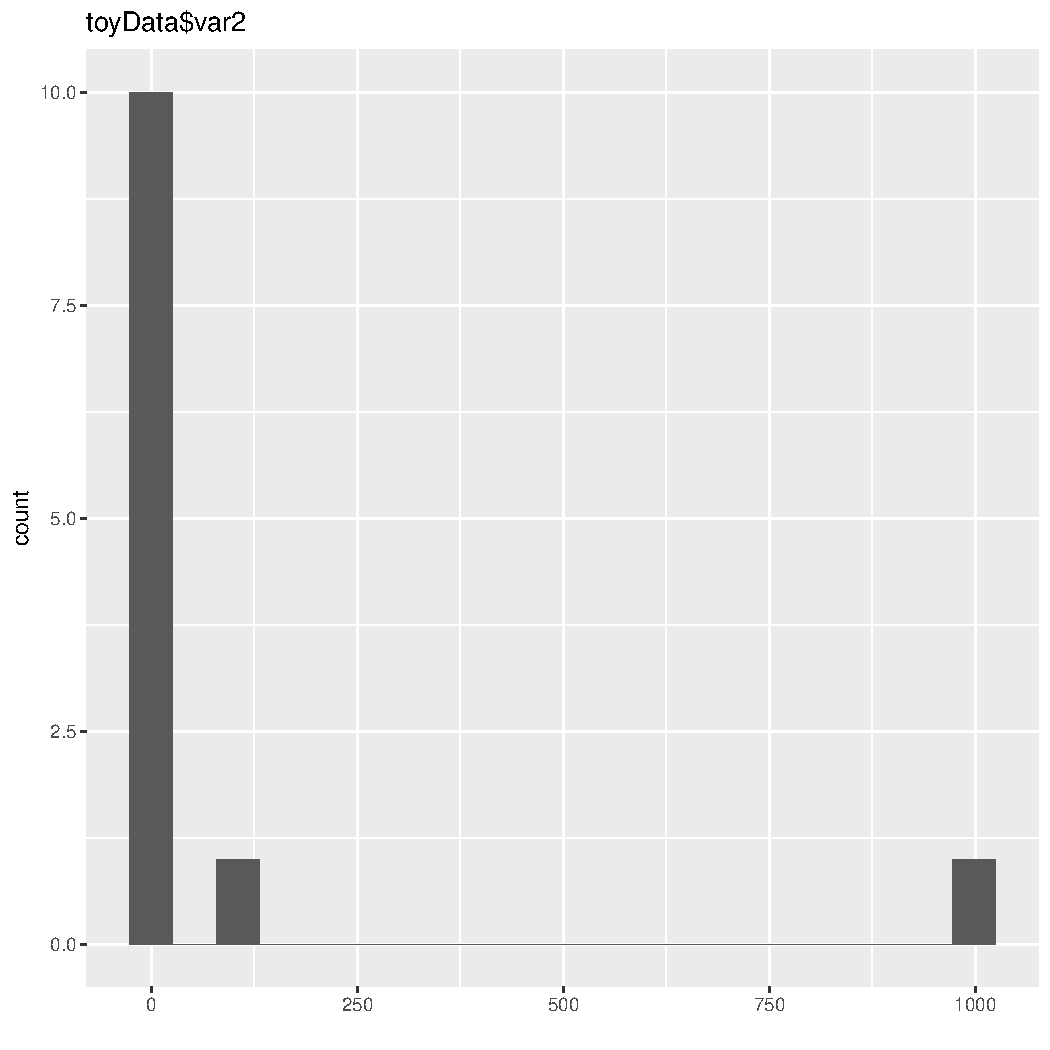
\includegraphics[width=7.5cm]{toyData-var2.pdf}
\end{center}
\caption{Output from running \code{visualize()} on the variable \code{var2} from the
\code{toyData} dataset.}
\label{fig:example2}
\end{figure}


As we saw with the \code{check()} function, the summary can be modified
by providing the relevant \code{XXXSummaries} arguments. Setting the
\code{numericSummaries} argument, we can control the summary output by
providing a vector of function names to run for a particular summary. To
only get the median, minimum and the maximum we set
\code{numericSummaries = c("centralValue", "minMax")}:

\begin{Schunk}
\begin{Sinput}
R> summarize(toyData$var2, numericSummaries = c("centralValue", "minMax"))
\end{Sinput}
\begin{Soutput}
     Feature         Result 
[1,] "Median"        "4"    
[2,] "Min. and max." "1; 82"
\end{Soutput}
\end{Schunk}

Note that the \code{summarize()}, \code{check()} and \code{visualize()} functions are also available interactively for full datasets by calling e.g., \code{summarize(toyData)}. However, this produces an extensive amount of output in the console, and therefore, we generally do not recommend it, unless working with very small datasets or subsets of datasets.

%\hl{
%\begin{itemize}
%\item Do an example with visualize() and summarize(), like the one with check(). Especially visualize and to doEval = T thing needs a bit of special attention.
% \item  Mention allCheckFunctions() etc. again here
% \item Mention check(), visualize() and summarize() modes for data.frames. Maybe also advice against it, at it will often produce a lot of information at once, and such large amounts of information really should be documented.
%\end{itemize}
%}

\section[Extending dataMaid]{Extending \pkg{dataMaid}}
\label{sec:extending}

\pkg{dataMaid} can be used as a user-friendly, self-contained package, as
shown in the previous sections. However, \pkg{dataMaid} is fully
customizable and \code{clean()} is mainly a tool for formatting the
results from various checking, summary,  and visualization
functions. Thus, the actual work underlying a \pkg{dataMaid} output file
can be anything --- depending on the arguments given to \code{clean()}
--- and user made functions are easily added to the
summarize/visualize/check-function arguments, as discussed previously.
However, the functions used in the SVC steps must adhere
to specific structures in order to be called from these three steps, and
therefore, we will now present how \code{summaryFunction}s,
\code{visualFunction}s and \code{checkFunction}s are made.


This section consists of two parts. First, we describe how customized
\code{summaryFunction}s, \code{visualFunction}s and
\code{checkFunctions} can be made, including an introduction to a few
convenient tools available in \pkg{dataMaid} for aiding SVC-function
construction.  Table \ref{table.functionTypes} serves as an overview
of the internals of these three central function types. Secondly, we
turn to a worked example of how to use custom made functions in
practice; Four new SVC functions are defined and used, both
interactively and in \code{clean()}.

\begin{table}[htbp]
\footnotesize
\bgroup
\def\arraystretch{1.8}%
\begin{tabular}{L{0.2\linewidth}L{0.2\linewidth}L{0.2\linewidth}L{0.2\linewidth}}
& \code{summaryFunction} & \code{visualFunction} & \code{checkFunction} \\
\hline
\vspace{0pt} Input (required) & \code{v} --- a variable vector.
                                \newline \code{...} --- additional
                                arguments passed to the function.  &  \code{v} --- a variable vector. \newline \code{vnam} --- the variable name (as character string). \newline \code{doEval} --- a logical (\code{TRUE}/\code{FALSE}) controlling the output type of the function. & \code{v} - a variable vector \newline \code{nMax} - an integer (or \code{Inf}), controlling how many problematic values are printed, if relevant \newline \code{...} --- additional arguments passed to the function. \\
Input (optional) &  \code{maxDecimals} --- number of decimals printed in outputted numerical values.  & --- &  \code{maxDecimals}  --- number of decimals printed in outputted numerical values.  \\
Purpose & Describe some aspect of the variable, e.g., a central value, its dispersion or level of missingness. & Produce a distribution plot. & Check a variable for a specific issue and, if relevant, identify the values in the variable that cause the issue. \\
Output (required) & A list with entries: \newline \code{\$feature} --- a label for the summary value (as character string); \newline \code{\$result} --- the result of the summary (as character string). & A character string with \proglang{R} code for producing a plot. This code should be standalone, i.e., should include the data if necessary. & A list with entries: \newline \code{\$problem} --- a logical identifying whether an issue was found; \newline \code{\$message} --- a character string (possibly empty) decribing the issue that was found, properly escaped and ready for use with \code{rmarkdown}. \\
Output (recommended) & A \code{summaryResult} object, i.e., an attributed list with entries \code{\$feature}, \code{\$result} and \code{\$value}, the latter being the values from \code{\$result} in their original format). & \bgroup
\def\arraystretch{1.8}%
\hspace*{-.2cm}\begin{tabular}[t]{p{0.45\linewidth} |
                 p{0.45\linewidth}} \vspace*{-1cm}\raggedright If
                 \code{doEval} is \code{TRUE}: \newline A plot that is
                 opened by the graphic device in \proglang{R}. &
                                                          \vspace*{-1cm}\raggedright If \code{doEval} is \code{FALSE}: \newline   A text string with \proglang{R} code, as described above. \end{tabular} \egroup  & A \code{checkResult} object, i.e., an attributed list with entries \code{\$problem}, \code{\$message} and \code{\$problemValues}, the latter being either \code{NULL} or the problem causing values, as they were found in \code{v}, whichever is relevant. \\
Tools available for producing the function & \code{summaryResult()} & --- & \code{messageGenerator()} \newline \code{checkResult()}
\end{tabular}
\egroup
\caption{Reference information for creating new functions to be used
  as part of the summarize, visualize, and check steps. The three
  columns correspond to each of the three function types. %\hl{I think the formatting here is still sort of chaotic. Maybe include horizontal lines everywhere? Is it allowed in JSS? It's impossible to read what's in which row right now.}
}
\label{table.functionTypes}
\end{table}



\subsection{Function templates}
\label{sec:functionTemplates}
In order to construct a summary, visual or check function, one needs
to create a new function with a specific structure.  This can be done with
different levels of strictness. If
the new custom function is only to be used as part of the SVC steps in \code{clean()},
then only the input/output structure of the function needs special attention.
However, new user-defined functions can also be registered locally to
be part of the full machinery of \pkg{dataMaid}, and these function will
be recognized and behave in the same way as the build-in functions in
\pkg{dataMaid}. The presentation below is given in the format of
function templates, written in pseudo-code. These templates are
designed for getting the full functionality, but note that
Table~\ref{table.functionTypes} serves as a reference to the minimal
requirements, while also presenting the "full" versions of the
function types.

% \hl{metatext, mention Table \ref{table.functionTypes} again.}

\subsubsection{Writing a summaryFunction}
As mentioned above, \pkg{dataMaid} provides a dedicated class for
\code{summaryFunction}s. However, this does not imply that they are
particularly advanced or complicated to create; in fact, they are
nothing but regular functions with a particular
input/output-structure. Specifically, they all follow the template
below:
\begin{Verbatim}
mySummaryFunction <- function(v, ...) {
  res <- [result of whatever summary we are doing]
  summaryResult(list(feature = "[Feature name]", result = res))
}
\end{Verbatim}
The last function called here, \code{summaryResult()}, changes the
class of the output, thereby making a \code{print()} method available
for it.  Note that \code{v} is an input vector and that \code{res}
should be either a character string or something that will be printed
as one. In other words an integer would be allowed, but a matrix will
not. Though a lot of different things can go into the
\code{summaryFunction} template, we recommend only using it for
summarizing the features of a variable, and leaving tests and checks
for the \code{checkFunction}s (presented below).

Adhering to the template above is sufficient for using the freshly
made \code{mySummaryFunction()} in \code{clean()}, but we recommend
adding the new function to the overview of all summary
functions by converting it to a proper \code{summaryFunction}
object. This is done by calling the \code{summaryFunction()} creator with
the user-defined function as the first argument, and additional arguments
\code{description} (an explanatory text which will be added to the attributes of
the function), and \code{classes} (a vector of variable classes the
user-defined function is intended to be applied to, also stored as an
attribute). In other words, a call following the template below should be made:
\begin{Verbatim}
mySummaryFunction <- summaryFunction(mySummaryFunction,
  description = "[Text describing what the summaryFunction does]",
  classes = c([vector of data types that the function is intended
  for]))
\end{Verbatim}
which adds the new function to the output of an
\code{allSummaryFunctions()} call.
% One comment should be devoted to
% the two attributes of a \code{summaryFunction}.
If the \code{description} argument is left unspecified, the name of
the function (which in this case is \code{"mySummaryFunction"}) will
be filled in and used as the \code{description} attribute. What
happens if the \code{classes} argument is not specified depends on the
type of \code{summaryFunction}. If \code{mySummaryFunction} is
constructed as an \code{S3} generic function with associated methods,
the call to \code{summaryFunction()} will automatically produce a
vector of the names of the classes for which the function can be
called. If \code{mySummaryFunction()} is not an \code{S3} generic and
\code{classes} is left unspecified, the attribute will simply be left
empty. Note that the helper function \code{allClasses()} might be
useful for filling out the \code{classes} argument, as it simply lists
all available classes in \pkg{dataMaid}:

\begin{Schunk}
\begin{Sinput}
R> allClasses()
\end{Sinput}
\begin{Soutput}
[1] "character" "Date"      "factor"    "integer"   "labelled" 
[6] "logical"   "numeric"  
\end{Soutput}
\end{Schunk}

% \hl{Write something here, don't end paragraph with code. Also, maybe move the allClasses() stuff somewhere else, it doesn't really belong under this header. Not sure where to, though.}


%Jeg foreslår at droppe nedenstående, da jeg synes det bliver lidt søgt i forhold
%til at det kun er beskrevet i pseudokode. (fx. er classes = numeric meget arbitrært)
%If we run the \code{allSummaryFunctions()} function we can see that the
%new function has been registered (output slightly appreviated):

%\begin{Schunk}
%\begin{Sinput}
%> allSummaryFunctions()
%\end{Sinput}
%\begin{Soutput}
%----------------------------------------------------------------------------
%name                description                                      classes
%------------------- --------------------------------------------------------
%mySummaryFunction   [Text describing what the summaryFunction does]  numeric
%.
%.
%.
%\end{Soutput}
%\end{Schunk}



\subsubsection{Writing a visualFunction}
\code{visualFunction}s are the functions that produce the figures in a
\pkg{dataMaid} output document. Writing a \code{visualFunction} is slightly
more complicated than writing a \code{summaryFunction}. This follows from
the fact that \code{visualFunction}s need to be able to output standalone
code for plots in order for \code{clean()} to build standalone
\pkg{rmarkdown} files. We recommend using the following structure
(again shown as pseudo code):
\begin{Verbatim}
myVisualFunction <- function(v, vnam, doEval) {
  thisCall <- call("[the name of the function used to produce the plot]",
    v, [additional arguments for the plotting function])
  if (doEval) {
    return(eval(thisCall))
  } else return(deparse(thisCall))
}
\end{Verbatim}

In this function, \code{v} is the variable to be visualized,
\code{vnam} is its name (which should generally be passed to
\code{title} or \code{main} arguments in plotting functions) and
\code{doEval} controls whether the output is a plot (if \code{TRUE})
or a character string of standalone code for producing a plot (if
\code{FALSE}). Implementing the \code{doEval = TRUE} setting is not
strictly necessary for a \code{visualFunction}'s use in \code{clean()}, but
it makes it easier to assess what visualization options are available,
and obviously, it is crucial for interactive usage of
\code{myVisualFunction()}. In either case, it should be noted that all
the parameters listed above, \code{v}, \code{vnam} and \code{doEval},
are mandatory, so they must be left as is, even if they are not in
use (c.f., Table~\ref{table.functionTypes}).


As with the summary function, we call \code{visualFunction()} to
register our newly created function:
%. Like before, it accepts the
%user-defined function as the first argument, and two additional
%arguments description which adds explanatory flavour text as an
%attribute of the function, and a vector which determines which classes
%the user-defined function should be applied to (which is also stored
%as an attribute).
\begin{Verbatim}
myVisualFunction <- visualFunction(myVisualFunction,
  description = "[Some text describing the visualFunction]",
  classes = c([data types that this function is intended for]))
  )
\end{Verbatim}

Now, \code{myVisualFunction()} will be available in a \code{allVisualFunctions()}
call, just like the two build-in \code{visualFunction}s, \code{standardVisual}
and \code{basicVisual}.

\subsubsection{Writing a checkFunction}
The last, but perhaps most important, \pkg{dataMaid} function type is
the \code{checkFunction}. These are the functions that flag issues in
the data as part of the check step and/or control the overall flow of the data
cleaning process in the pre-check stage. A \code{checkFunction} follows
one of two overall structures, depending on the type of check. Either,
it tries to identify problematic values in the variable (as
e.g., \code{identifyMissing()} does), or it performs a check concerning the
variable as a whole (e.g., the functions used for pre-checks and the
function \code{identifyNums()}). We present templates for both types of
\code{checkFunction}s below separately, but it should be emphasized that
formally, they belong to the same class.

First, a template for the full-variable check function type, where we
first define the function and subsequently register it as a check
function using \code{checkFunction()}:
\begin{Verbatim}
myFullVarCheckFunction <- function(v, ...) {
  [do your check]
  problem <- [is there a problem? TRUE/FALSE]
  message <- "[message describing the problem, if any]"
  checkResult(list(problem = problem,
    message = message,
    problemValues = NULL))
}

myFullVarCheckFunction <- checkFunction(myFullVarCheckFunction,
  description = "[Some text describing the checkFunction]",
  classes = c([the data types that this function is intended to be used for])
  )
\end{Verbatim}

Again, as with \code{summaryFunction}s and \code{visualFunction}s, the
change of function class by use of \code{checkFunction()} is not strictly
necessary. Note however, that if \code{myFullVarCheckFunction} is to be
used in the summarize/visualize/check steps in \code{clean()}, the
description attribute will be printed in the overview table in the
\textit{Data cleaning summary} part of the output document.

If problematic values are to be identified, the template from above
should be expanded to follow a slightly more complicated structure
(again shown as pseudo-code):

\begin{Verbatim}
myProbValCheckFunction <- function(v, nMax, maxDecimals, ...) {
  [do your check]
  problem <- [is there a problem? TRUE/FALSE]
  problemValues <- [vector of values in v that are problematic]
  problemStatus <- list(problem = problem,
                        problemValues = problemValues)

  problemMessage <- "[Message that is printed prior to listing
                     problem values in the dataMaid output,
                     ending with a colon]"

  outMessage <- messageGenerator(problemStatus, problemMessage, nMax)

  checkResult(list(problem = problem,
    message = outMessage,
    problemValues = problemValues))
}

myProbValCheckFunction <- checkFunction(myProbValCheckFunction,
  description = "[Some text describing the checkFunction]",
  classes = c([the data types that this function is intended to be used for])
)
\end{Verbatim}

One comment should be devoted to the helper function,
\code{messageGenerator()}.  This function's sole purpose is aiding
consistent styling of all \code{checkFunction} messages. The function
simply pastes together the \code{problemMessage} and the
\code{problemValues}, with the latter being quoted and sorted
alphabetically. If the \code{nMax} argument to \code{messageGenerator()} is
not \code{Inf}, only the first \code{nMax} problem values will be pasted
onto the message, accompanied by a comment about how many problem
values were left out (if any).  Note that printing quotes in
\proglang{R} markdown requires an extensive amount of character escaping, so
opting for \code{messageGenerator()} really is the easiest solution.

In the template above, the argument \code{maxDecimals} is not in use. This
argument should be used to round off the \code{problemValues} passed to
\code{messageGenerator()}, if they are numerical.  This can be done by
adding an extra line of code after defining \code{problemStatus} in the template
above:

\begin{Verbatim}
myProbValCheckFunction <- function(v, nMax, maxDecimals, ...) {
  [... more lines of code here ...]
  problemStatus <- list(problem = problem,
    problemValues = problemValues)

  if (!is.null(problemValues)) {
    problemStatus$problemValues <- round(problemValues, maxDecimals)
  }
  [... more lines of code here ...]
}
\end{Verbatim}
% $

Now, problematic values will be rounded in the outputted message, while they
will still appear in their original format under the entry \code{\$problemValues} %$
in the returned object.

\subsection{A worked example}

As an example, we create four new functions and show both how they can be
used interactively and how they can be integrated with the \code{clean()}
function. These four new functions are:
\begin{description}
\item[\code{isID()}] A new \code{checkFunction} intended for use in the pre-check-stage. This function checks whether a variable consists exclusively of long ($> 10$ characters/digits) entries that are all of equal length, as this might be personal identification codes that we do not wish to print out in the data summary.
\item[\code{mosaicVisual()}] A new \code{visualFunction} that produces mosaic plots. This function will be used in the \textit{visualize} step of \code{clean()}.
\item[\code{countZeros()}] A new \code{summaryFunction} that counts the number of occurrences of the value \code{0} in a variable. This function will be used in the \textit{summarize} step of \code{clean()}.
\item[\code{identifyColons()}] A new \code{checkFunction} that flags variables in which values have colons that appear before and after alphanumerical characters. This is practical for identifying autogenerated interaction effects. This function will be used in the \textit{check} step of \code{clean()}.
\end{description}
These functions are defined in turn below, and afterwards, an example of how they can be called from \code{clean()} is provided.

\subsubsection[isID --- a new checkFunction without problem values]{\code{isID} --- a new \code{checkFunction} without problem values}
First, let's define the \code{isID()} function. As this function is
not supposed to list problematic values, it falls within the category
of \code{checkFunction}s represented by
\code{myFullVarCheckFunction()} above. We do not particularly wish to
use this function interactively, so we will stick to the minimal
requirements of a \code{checkFunction} used in \code{check()} (see
Table~\ref{table.functionTypes}). The function can then be defined by

\begin{Schunk}
\begin{Sinput}
R> isID <- function(v, nMax = NULL, ...) {
+    out <- list(problem = FALSE, message = "")
+    if (class(v) %in% setdiff(allClasses(), c("logical", "Date"))) {
+      v <- as.character(v)
+      lengths <- c(nchar(v))
+      if (all(lengths > 10) & length(unique(lengths)) == 1) {
+        out$problem <- TRUE
+        out$message <- "Warning: This variable seems to contain ID codes."
+      }
+    }
+    out
+  }
\end{Sinput}
\end{Schunk}

This is essentially all we need to do in order to include this
function as a pre-check-function in \code{clean()}, so we will leave it as
is and move on to the next function, namely \code{mosaicVisual()}.

\subsubsection[mosaicVisual --- a new visualFunction]{\code{mosaicVisual} --- a new \code{visualFunction}}
\proglang{R} provides a function, \code{mosaicplot()}, which produces
mosaic plots. We intend to use this existing high-level plotting
function as part of the new visualization function.  We will define
the new function such that it gets the full \pkg{dataMaid}
functionality. This can be done using the following code which sets up
the call using the existing function \code{mosaicplot()}.

\begin{Schunk}
\begin{Sinput}
R> mosaicVisual <- function(v, vnam, doEval) {
+    thisCall <- call("mosaicplot", table(v), main = vnam, xlab = "")
+    if (doEval) {
+      return(eval(thisCall))
+    } else return(deparse(thisCall))
+  }
\end{Sinput}
\end{Schunk}

This function can now be called directly or used in \code{clean()}, as will
presented in an example below. Depending on the \code{doEval} argument, either a text string
with code or a plot is produced. The plot resulting from the following
call is found in Figure~\ref{fig:mosaicPlot}:

\begin{Schunk}
\begin{Sinput}
R> mosaicVisual(toyData$var1, "variable 1", doEval = TRUE)
\end{Sinput}
\end{Schunk}

\begin{figure}
\begin{center}
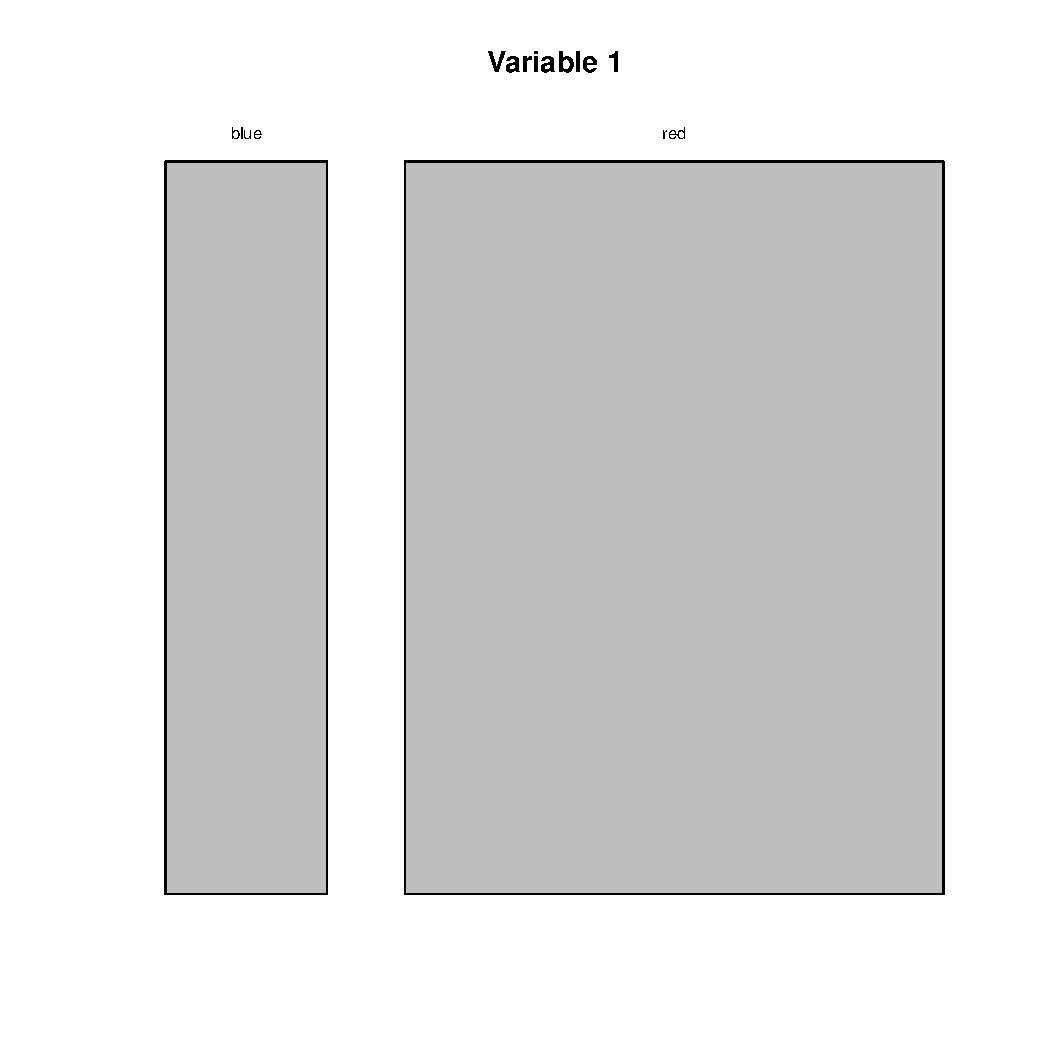
\includegraphics[scale=0.2]{mosaicPlotExample.pdf}
\end{center}

\caption{Mosaic plot generated by the user-defined visualization
  function \code{mosaicVisual()}.}
\label{fig:mosaicPlot}
\end{figure}




Even though \code{mosaicVisual()}, as written above, follows the style of a
\code{visualFunction}, it is not yet truly one and therefore, it will not
appear in an \code{allVisualFunctions()} call. In order to get this
functionality we need to change its object class. This can be done by
writing

\begin{Schunk}
\begin{Sinput}
R> mosaicVisual <- visualFunction(mosaicVisual,
+    description = "Mosaic plots using graphics",
+    classes = allClasses())
\end{Sinput}
\end{Schunk}

Here, we use the function \code{allClasses()} to quickly obtain a vector
of all the seven variable classes addressed in \pkg{dataMaid}. Note that
if \code{mosaicVisual()} were an S3 generic function, this argument could
have been left as \code{NULL} and then the classes for which methods are
available would be added automatically.
%\hl{I'm repeating myself here,
%  but I think it is quite a neat feature, so maybe that's okay?}

As \code{mosaicVisual()} is now a full-blooded \code{visualFunction}, it
will also be included in the \code{allVisualFunctions()} output table:
\begin{Schunk}
\begin{Sinput}
R> allVisualFunctions()
\end{Sinput}
\begin{Soutput}
------------------------------------------------------------------------------
name             description                     classes                      
---------------- ------------------------------- -----------------------------
mosaicVisual     Mosaic plots using graphics     character, Date, factor,     
                                                 integer, labelled, logical,  
                                                 numeric                      

basicVisual      Histograms and barplots using   character, Date, factor,     
                 graphics                        integer, labelled, logical,  
                                                 numeric                      

standardVisual   Histograms and barplots using   character, Date, factor,     
                 ggplot2                         integer, labelled, logical,  
                                                 numeric                      
------------------------------------------------------------------------------
\end{Soutput}
\end{Schunk}

Now that we are done with the definition of \code{mosaicVisual()} we can
turn to the next function in line, \code{countZeros()}.

\subsubsection[countZeros --- a new summaryFunction]{\code{countZeros} --- a new \code{summaryFunction}}
This \code{summaryFunction} is defined in the following lines of code:

\begin{Schunk}
\begin{Sinput}
R> countZeros <- function(v, ...) {
+    res <- length(which(v == 0))
+    summaryResult(list(feature = "No. zeros", result = res, value = res))
+  }
\end{Sinput}
\end{Schunk}

As this function computes an integer (the number of zeros),
there is no difference between the elements \code{\$result} and
\code{\$value}. If, on the other hand, the result had been a character
string, extra formatting might be required in the \code{\$result} entry
(such as escaping of quotation marks), and in this scenario, the two
entries would have differed. As the result is returned as a
\code{summaryResult} object, a printing method is automatically called
when \code{countZeros()} is used interactively:

\begin{Schunk}
\begin{Sinput}
R> countZeros(c(rep(0, 5), 1:100))
\end{Sinput}
\begin{Soutput}
No. zeros: 5
\end{Soutput}
\end{Schunk}

As with \code{mosaicVisual()}, we change the class of this function in
order to make it appear in \code{allSummaryFunctions()} calls. But now we
wish to emphasize that the function is not intended to be called on
all variable types, as zeros have different roles in \code{Date}s and in
\code{logical} variables:

\begin{Schunk}
\begin{Sinput}
R> countZeros <- summaryFunction(countZeros,
+    description = "Count number of zeros",
+    classes = c("character", "factor", "integer",
+    "labelled", "numeric"))
\end{Sinput}
\end{Schunk}

\subsubsection[identifyColons --- a new checkFunction with problem values]{\code{identifyColons} --- a new \code{checkFunction} with problem values}
The last function mentioned above is \code{identifyColons()}. We
define it using the helper function \code{messageGenerator()} to
obtain a properly escaped message, and we use \code{checkResult()} to
make its output print neatly. In the code we use regular expressions
through the \code{gregexpr()} function to identify colons between two
words.

\begin{Schunk}
\begin{Sinput}
R> identifyColons <- function(v, nMax = Inf, ... ) {
+    v <- unique(na.omit(v))
+    problemMessage <- "Note: The following values include colons:"
+    problem <- FALSE
+    problemValues <- NULL
+  
+    problemValues <- v[sapply(gregexpr("[[:xdigit:]]:[[:xdigit:]]", v),
+      function(x) all(x != -1))]
+  
+    if (length(problemValues) > 0) {
+      problem <- TRUE
+    }
+  
+    problemStatus <- list(problem = problem,
+      problemValues = problemValues)
+  
+    outMessage <- messageGenerator(problemStatus, problemMessage, nMax)
+  
+    checkResult(list(problem = problem,
+      message = outMessage,
+      problemValues = problemValues))
+  }
\end{Sinput}
\end{Schunk}

Once again, we change the class of the function so that it becomes a
proper \code{checkFunction} object:

\begin{Schunk}
\begin{Sinput}
R> identifyColons <- checkFunction(identifyColons,
+    description = "Identify colons surrounded by alphanumeric characters",
+    classes = c("character", "factor", "labelled"))
\end{Sinput}
\end{Schunk}

Note, that for \code{checkFunction}s, the description will appear in
the document produced by \code{clean()} (in the \textit{Data cleaning
  summary} section of the output), so for this type of function, the
change of class is not only done for the sake of the
\code{allCheckFunctions()} output.

\subsubsection[Calling the new summarize/visualize/check functions from clean()]{Calling the new summarize/visualize/check functions from \code{clean()}}
Now, we are ready to use these new functions in a \code{clean()}
call. The extended \pkg{dataMaid} output document should have the
following modifications, relative to the standard \pkg{dataMaid} output:
\begin{itemize}
\item We want to add the new pre-check function, \code{isID()}, to the already existing pre-checks.
\item We wish to change the plot type for all variables to the new mosaic plot.
\item We want the new summary function, \code{countZeros()}, to be added to the summaries performed on all variable types but \code{Date} and \code{logical}.
\item We want the new check function, \code{identifyColons()}, to be added to the checks performed on \code{character}, \code{factor} and \code{labelled} variables.
\end{itemize}
These options are specified as follows:

\begin{Schunk}
\begin{Sinput}
R> data("exampleData")
R> clean(exampleData,
+    preChecks = c("isKey", "isEmpty", "isID"),
+    allVisuals = "mosaicVisual",
+    characterSummaries = c(defaultCharacterSummaries(), "countZeros"),
+    factorSummaries = c(defaultFactorSummaries(), "countZeros"),
+    labelledSummaries = c(defaultLabelledSummaries(), "countZeros"),
+    numericSummaries = c(defaultNumericSummaries(), "countZeros"),
+    integerSummaries = c(defaultIntegerSummaries(), "countZeros"),
+    characterChecks = c(defaultCharacterChecks(), "identifyColons"),
+    factorChecks = c(defaultFactorChecks(), "identifyColons"),
+    labelledCheck = c(defaultLabelledChecks(), "identifyColons"))
\end{Sinput}
\end{Schunk}

The outputted document is found in Appendix \ref{sec:appendix2}.

\section{Rubbing down data cleaning challenges}
\label{sec:specificExamples}
%\hl{Lidt poppet titel, men den gamle ("Using dataMaid in specific situations")
%fik mig til flabel at tænke "i modsætning til uspecifikke situationer?". Jeg
%er dog meget åben for en bedre titel.}

Finally, we present a few examples of how to make \pkg{dataMaid}
solve specific issues related to data cleaning. First, we discuss the
challenges related to cleaning large datasets, particularly in terms
of memory use and computation speed. Next, we show how \pkg{dataMaid}
can be used for problem-flagging. Lastly, we discuss how the
\pkg{dataMaid} output document can be included in other \proglang{R} markdown
documents as a way to produce clear and concise documentation of a
dataset. %\hl{I feel like there should be more topics here, but I'm all
%  out of ideas...}

\subsection{Cleaning large datasets}
If the dataset becomes very large, the standard use of \code{clean()}
outlined above might not be ideal. If there is a large number of
variables, creation of the \proglang{R} markdown document might be quite
slow, while a large number of observations will generally affect the
rendering time of the document. This issue is especially relevant to
Windows users, where memory usage is not very efficient. The problem is that older,
32-bit versions of Windows generally cannot access all physical RAM,
while newer 64-bit versions of Windows cannot access virtual memory. Therefore,
memory allocation issues becomes even more pressing under Windows.

Below we give a few practical examples of ways to deal with large
data, while wishing to still produce (potentially very long) data
cleaning overview documents. Note that the interactive tools of
\pkg{dataMaid} can be used as usual or sequentially in small subsets
of the large dataset, if no overview documents are needed.

\subsubsection{Handling the figures}
Though figures give a nice overview of each variable, they are also
quite heavy objects in terms of memory allocation. Therefore, it might
be beneficial to not include figures in the \pkg{dataMaid} outputs for
very large datasets. This is controlled via the \code{mode} argument:

\begin{Schunk}
\begin{Sinput}
R> clean(toyData, mode = c("summarize", "check"))
\end{Sinput}
\end{Schunk}

If figures are indeed needed, a different approach is to choose the
less memory heavy standard \proglang{R} figure style instead of the
\pkg{ggplot2} figures that are the default option in \code{clean()}. This
can be done by setting the \code{allVisuals = "basicVisual"} argument:

\begin{Schunk}
\begin{Sinput}
R> clean(toyData, allVisuals = "basicVisual")
\end{Sinput}
\end{Schunk}

Of course, even less heavy plots might be achieved by writing new
\code{visualFunction}s, using the guidelines from Section
\ref{sec:functionTemplates}. For instance, a future extension of
\pkg{dataMaid} might be the inclusion of ASCII plots, as
e.g., represented in the \proglang{R} package \pkg{txtplot} \citep{txtplot}.

%\hl{I really feel like we should do some benchmarking here, maybe just on toyData, both in terms of speed and memory use. I would make the recommendations more trustworthy and serious.}

\subsubsection{Economic memory use}
Another solution, which is
especially relevant to Windows users due to %the unfortunate
the memory handling on this operating system,
%combination of memory control in this operating system and
%\proglang{R},
is simply splitting the two steps performed
by \code{clean()}, namely producing the \proglang{R} markdown file and rendering it
afterwards. If the \code{rmarkdown} file is very long, as it will
typically be for very large datasets, keeping this file open in memory
wastes precious memory capacities. Therefore, we advice users to
instead split the two steps as shown in the following.

\begin{Schunk}
\begin{Sinput}
R> clean(toyData, render = FALSE, openResult = FALSE)
R> render("dataMaid_toyData.Rmd", quiet = FALSE)
\end{Sinput}
\end{Schunk}

This also deals with the fact that \pkg{dataMaid} can produce
\proglang{R} markdown files that supersedes the upper size limit of code editors, e.g.,
RStudio, which currently has an editor file size limit of 5MB. %\hl{dette giver
%ingen mening uden en præcision? "upper size limit" af hvad? Se udkommenteret
%kommentar.}
% of RStudio,
%which is currently \hl{find number} GBs (using RStudio version
%1.0.44).
%\hl{Is this maybe too editor specific? On the other hand, a
%  lot of people do use RStudio...}.

\subsection[Using dataMaid for problem flagging]{Using \pkg{dataMaid} for problem flagging}
If the data is large, but memory issues and computation time are less
of an issue than the time it takes a human to look through the data
cleaning document, a viable solution might be not to include all
information about all variables. % Or even for more reasonably sized
% datasets, sometimes a brief overview of the most pressing issues can
% be useful.
This can be achieved by using the \code{onlyProblematic} argument in
\code{clean()}. By specifying \code{onlyProblematic = TRUE}, only
variables that raise a flag in the checking steps will be summarized
and visualized. But perhaps we are not even interested in obtaining
general information about these variables, but only in getting a quick
overview of the problems they might have. This is obtained by
controlling the \code{mode} argument:

\begin{Schunk}
\begin{Sinput}
R> clean(toyData, onlyProblematic = TRUE, mode = c("check"))
\end{Sinput}
\end{Schunk}

Now only the checking results are printed, and only for variables
where problems were identified. An even more minimal output can be
generated by also leaving out the checking results --- then
\code{clean()} essentially just produces a document with a list of the variable names
that should be investigated further:

\begin{Schunk}
\begin{Sinput}
R> clean(toyData, onlyProblematic = TRUE, mode = NULL)
\end{Sinput}
\end{Schunk}

Of course, this can also be done without generating an overview
document, by direct, interactive use of the \code{check()} function. When
called on a \code{data.frame}, this function produces a list (of
variables) of lists (of checks) of lists (or rather,
\code{checkResult}s). Thus, the overall problem status of each variable
can easily be unravelled using the list manipulation function
\code{sapply()}:

\begin{Schunk}
\begin{Sinput}
R> toyChecks <- check(toyData)
R> foo <- function(x) {
+    any(sapply(x, function(y) y[["problem"]]))
+  }
R> sapply(toyChecks, foo)
\end{Sinput}
\begin{Soutput}
 var1  var2  var3  var4  var5  var6 
 TRUE  TRUE  TRUE  TRUE  TRUE FALSE 
\end{Soutput}
\end{Schunk}

and we find that only a single variable in \code{toyData}, \code{var6} (for which all
observations have the value \code{"Irrelevant"}), is problem-free.


\subsection[Including dataMaid documents in other files]{Including \pkg{dataMaid} documents in other files}
Sometimes, a \pkg{dataMaid} document might be a useful addition to a
more general overview document, including additional information such
as pairwise association plots, time series plots, or exploratory
analysis results.  \pkg{dataMaid} can produce a document to be
included in other \proglang{R} markdown files by setting the
\code{standAlone} argument in \code{clean()} to remove the preamble
from the output \proglang{R} markdown file. Note that it is still
necessary to indicate which \proglang{R} markdown output type is
created; the pdf and html \proglang{R} markdown styles are
unfortunately not identical.

If it is important that the embedded \pkg{dataMaid} document can be
rendered to either of these two file types, we recommend setting
\code{twoCols = FALSE} and \code{output = "html"} in \code{clean()}, thereby
essentially removing almost all output type specific formatting code
from the generated \proglang{R} markdown file.

On the other hand, if a pdf document is to be produced, a few extra
lines need to be added to the preamble of the master \proglang{R} markdown
document --- otherwise, the two-column layout code will produce an
error. The following is an example of how such a master document
preamble YAML might look like and how the \code{dataMaid\_toyData.Rmd} file can
then be included:

{\small
\begin{Verbatim}
---
output: pdf_document
documentclass: report
header-includes:
  - \renewcommand{\chaptername}{Part}
  - \newcommand{\fullline}{\noindent\makebox[\linewidth]{\rule{\textwidth}{0.4pt}}}
  - \newcommand{\bminione}{\begin{minipage}{0.75 \textwidth}}
  - \newcommand{\bminitwo}{\begin{minipage}{0.25 \textwidth}}
  - \newcommand{\emini}{\end{minipage}}
---

```{r, child = 'dataMaid_toyData.Rmd'}
```
\end{Verbatim}
}
%\hl{Use proper formatting here. How do we do non-R code?}

In the this example, the \code{dataMaid\_toyData.Rmd} file could have
been created as follows:

\begin{Schunk}
\begin{Sinput}
R> clean(toyData, standAlone = FALSE)
\end{Sinput}
\end{Schunk}

and the more minimal, html-style \proglang{R} markdown file described above can be produced using

\begin{Schunk}
\begin{Sinput}
R> clean(toyData, standAlone = FALSE, output = "html", twoCols = FALSE)
\end{Sinput}
\end{Schunk}

Note that with the latter option, no special YAML preamble is needed in the \proglang{R} markdown document.
% \hl{don't end on code.}



\section{Concluding remarks}
\label{conclusion}
%\hl{Is this a thing in this journal? Otherwise, we might want to make some final remarks in the previous sections. Feels awkward to end with a bunch of code and some super specific examples...}

In this paper we have introduced the \proglang{R} package \pkg{dataMaid}
for performing reproducible error detection and data cleaning
summaries. The package provides a general and extendable framework for
identifying potential errors and for creating human-readable summary
documents that will help investigators to identify possible errors in
the data.


While the the current release is stable, the authors have an interest
in further developing the functionality of \pkg{dataMaid} by providing
more summary, visual, and check function as part of the default
package. We are also currently considering adding options to handle
repeated measurement, where the visualizations --- in particular ---
might be improved by visualizing measurements over time. In addition,
an online \pkg{shiny} \citep{shiny} application where users that are not
\proglang{R}-savvy can upload their data and get a data cleaning
document is currently planned.



% \nocite{R}
%\nocite{shiny}
%\nocite{dataMaid}
%\nocite{rmarkdown}
%\nocite{ggplot2}
%\nocite{plyr}
%\nocite{data.table}
%\nocite{validate}
%\nocite{editrules}
%\nocite{janitor}
%\nocite{DataCombine}
%\nocite{txtplot}

% \bibliographystyle{jss}
\bibliography{foo}


\appendix
\newpage

%\includepdf[scale=0.8,clip,trim=0cm 0cm 0cm
%2cm,pages={1},pagecommand={\section{appendix}\subsection{par‌​t1}}]{pdfdocument} \includepdf[sc%ale=0.8,clip,trim=0cm
%0cm 0cm 2cm,pages={2-5},pagecommand={}]{pdfdocument}

% \section{Appendix A: cleaning the toyData data frame} \label{sec:appendix1}
\includepdf[pages=2, pagecommand={\section{Appendix A: cleaning the toyData data frame} \label{sec:appendix1}}, frame=true, noautoscale=true, scale=0.7]{dataMaid_toyData.pdf}
\includepdf[pages=3-4, pagecommand={}, frame=true, noautoscale=true, scale=0.7,pagecommand={}]{dataMaid_toyData.pdf}



\includepdf[pages=2, pagecommand={\section{Appendix B: User-extended cleaning of
  exampleData} \label{sec:appendix2}}, frame=true, noautoscale=true, scale=0.7]{dataMaid_exampleData.pdf}
\includepdf[pages=3-, pagecommand={}, frame=true, noautoscale=true, scale=0.7]{dataMaid_exampleData.pdf}
%\hl{Data cleaning with user supplied extensions here}

\end{document}
